\subsubsection{In Person Evaluations}

\paragraph{Survey Design}
Evaluations were completed in person with 10 different volunteer students over 2 days.
The goal was to check on the ease of use of the new WolfTutor application; to make sure
the enhancements did not make the application any harder to use or slower in live-time. 
To determine how long a user would spend finding a tutor on the application, two missions were given
to the students. One, to find a tutor as a student who really wanted a tutor with a high GPA. Two, to find a tutor
as a student that really wanted a tutor with good reviews. Students were encouraged to take other factors into account
as well to make the simulation more realistic. To avoid bias, a coin was flipped to decide which WolfTutor system to start with - old or new.
This resulted in 6 users evaluating the old system before the new system. 

\paragraph{Results}
Out of the 10 students, 4 took longer to use the new WolfTutor application when searching for GPA. The largest time
increase was 31 seconds. When searching for a tutor with good reviews, a different set of 4 students took longer with the new
WolfTutor. The longest time increase was 56 seconds. Even though more users completed the time trials
for the old application first, the users that completed the new application's trials first only accounted for 4 of the 
12 time differences that resulted in the new application being faster.

Students were asked to provide the tutor that they chose during the time trials.
When filtering by GPA, there were a total of 8 different tutors chosen in the old appliaction and
only 3 in the new one. When filtering by reviews, 8 different tutors were chosen in the old and 5 were
chosen in the new. 

Students were also asked to provide a brief reasoning for why they chose their tutor.
For the new application and for the review filter on the old application, the responses vary between the qualities of a tutor
the student prioritizes. For example: major, level of degree, and price.  When filtering for GPA, some students still took reviews
into account because it was important to them. Not just having a high average rating, but having a better distribution of ratings such that there
were more high ratings. Since there is no GPA given on the old system, students were asked to try to pick a tutor 
based on whether they seemed like they would have a high GPA or that seemed to be the smartest. For the most part, the reasoning given
for choosing a tutor was random selection, although some students did take other qualities into account.
For example, choosing the tutor that had the highest degree level that they could find.

These results signify: 
\begin{itemize}
  \item that the new WolfTutor application does not break the system such that it lessens usability.
  \item the qualities that make a good tutor are controverisal and the application could use more filters
  \item the new WolfTutor helped make the better tutors more obvious, as the range of tutors chosen decreased.
\end{itemize}


\paragraph{Feedback}
At the beginning of the evaluation, students were asked if they had ever paid for a tutor in the past. Out of all 10 students,
6 had and 4 had not. Out of the 6 that had, 2 of them reported finding the tutors online. The other
4 either found their tutor through a friend's recommendation or the tutor was actually their friend. Since most
of them never used an online service for finding a tutor, there did not seem to be much bias. It also meant
the students did not have a better system in mind to offer additonal features that could be implemented in WolfTutor.
However, some students did make suggestions:
\begin{itemize}
  \item adding in a filter for price
  \item being able to demo with a tutor
  \item the ability to change the weights of the filters because they did not think GPA was that important
  \item a larger selection of tutors. This is addressed in section \ref{mock-data}
\end{itemize}



\subsubsection{Responding to Change}
\label{sec:change}
% TODO: Talk about the changes we made after the first round of tutori
The team performed evaluations in person and over two days.  At the end of
the first day, there were a few issues that had been consistently pointed out
that were fairly straightforward to fix.  To help focus on evaluating the speed
of use of the system, the team opted to fix a few of these issues immediately
before the second round of tutoring. In addition to these changes, section \ref{sec:mock}
discusses slight alterations made to the databases after evaluation day 1.

\begin{figure}
  \caption{The tutor display prompt for a volunteer.} \label{fig:tutor_display}
  \centering
    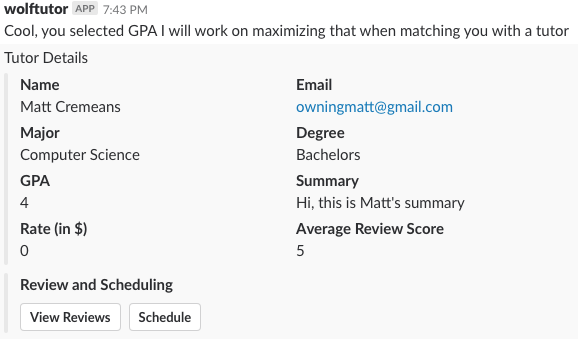
\includegraphics[width=0.5\textwidth]{tutor-display.png}
\end{figure}

% Fixed prompt to display rate as a currency
The first thing that was changed was a menu from the original system.  In the
original system, the tutor display had a "Rate'' section that was intended to
display that tutor's billing rate.  During our trials, testers consistently
mistook this for a rating, so the team made the decision to add the quantifier
added in figure \ref{fig:tutor_display} switch things out.

% Added average tutor score to tutor display
The team also decided to add one other menu item. During the initial
development, the team intended to add average tutor review score to the same
tutor display discussed above, but overlooked that simple enhancement at the
time.  This made it more difficult for students to actually run the tests,
though it was still possible through the use of the original ``review'' view.
This field is also visible in figure \ref{fig:tutor_display}.

% Fixed order of tutors display
The final major change made after the first round of tutoring was a bugfix.
During the first round of evaluations, the team realized that the tutors being
displayed were displaying out of order from what the team expected.  After
investigating, it was discovered that the suggestion algorithm was not
malfunctioning as originally thought, but that the Slack API used to send the
tutor suggestions to the users was delivering messages asynchronously, rather
than synchronously as had been thought during development and initial testing.
This was rectified by changing to a different interface that, while slower
because it performed a handshake with every message, delivered the messages in
the correct order.  

%%% Local Variables:
%%% mode: latex
%%% TeX-master: "../main"
%%% End:
